\chapter{Análisis de Algoritmos}

% ============================================================
% Paquetes necesarios (ya deberían estar en el preámbulo)
% \usepackage{amsmath, amssymb, amsthm}
% \usepackage{listings, xcolor}
% \usepackage{tcolorbox}
% \tcbuselibrary{skins, breakable}
% \usepackage{tikz}
% \usepackage{pgfplots}
% \pgfplotsset{compat=1.18}
% ============================================================

% Colores para el código Python
\definecolor{pyblue}{RGB}{0,0,255}
\definecolor{pygreen}{RGB}{0,128,0}
\definecolor{pyred}{RGB}{255,0,0}
\definecolor{pygray}{RGB}{128,128,128}
\definecolor{pyback}{RGB}{245,245,245}

\lstset{
  language=Python,
  basicstyle=\small\ttfamily,
  keywordstyle=\color{pyblue}\bfseries,
  commentstyle=\color{pygreen}\itshape,
  stringstyle=\color{pyred},
  numberstyle=\tiny\color{pygray},
  stepnumber=1,
  numbers=left,
  backgroundcolor=\color{pyback},
  frame=single,
  breaklines=true,
  tabsize=4,
  showspaces=false,
  showstringspaces=false,
  captionpos=b,
}

% Estilos para cajas de teoremas
\newtcolorbox{definicionBox}{
  colback=blue!5,
  colframe=blue!75!black,
  fonttitle=\bfseries,
  title=Definición,
  breakable
}

\newtcolorbox{observacionBox}{
  colback=yellow!5,
  colframe=yellow!75!black,
  fonttitle=\bfseries,
  title=Observación,
  breakable
}

\newtcolorbox{ejemploBox}{
  colback=green!5,
  colframe=green!75!black,
  fonttitle=\bfseries,
  title=Ejemplo,
  breakable
}

% Redefinir entornos existentes (si ya están definidos, comentar)
% Si ya tienes definiciones con \newtheorem, puedes usar las cajas manualmente
% o redefinirlas. En este caso, mantendré los nombres originales pero con cajas.
% Para no romper la compilación, asumo que en el preámbulo ya están definidos
% los entornos definicion, observacion, ejemplo. Si no, los creo aquí.
% Para simplificar, usaré directamente los entornos con tcolorbox.


% Renombrar los entornos para usar cajas
\renewenvironment{definicion}
  {\begin{definicionBox}}
  {\end{definicionBox}}

\renewenvironment{observacion}
  {\begin{observacionBox}}
  {\end{observacionBox}}

\renewenvironment{ejemplo}
  {\begin{ejemploBox}}
  {\end{ejemploBox}}


% ============================================================
% INICIO DEL CAPÍTULO
% ============================================================

\section{Introducción}

\begin{definicion}
La \textbf{demora temporal} de un algoritmo (comúnmente conocida como tiempo de ejecución o complejidad temporal) es una medida que estima o calcula el tiempo que tarda un algoritmo en completarse en función del tamaño de sus datos de entrada.
\end{definicion}

\begin{observacion}
\begin{itemize}
  \item No se mide típicamente en segundos o minutos, sino en el número de operaciones fundamentales (o pasos) que realiza. Esto se debe a que el tiempo real en segundos depende de factores externos como la velocidad del hardware, el lenguaje de programación o la carga del sistema.
  \item El tiempo de ejecución depende de los datos de entrada. En lugar de analizar entradas específicas, se usan parámetros que definen su tamaño; por ejemplo, si la entrada es un conjunto que contiene $n$ elementos, se diría que el tamaño de la entrada es $n$.
\end{itemize}

\textbf{Tipos de análisis de tiempo:}
\begin{itemize}
  \item \textbf{Mejor caso:} tiempo mínimo necesario para una entrada de tamaño $n$.
  \item \textbf{Peor caso:} tiempo máximo necesario para una entrada de tamaño $n$.
  \item \textbf{Caso promedio:} tiempo necesario para un conjunto representativo de entradas de tamaño $n$.
\end{itemize}
\end{observacion}

\begin{observacion}[Estimación vs. cálculo exacto]
El objetivo es obtener una medida útil del tiempo, no un cálculo preciso. Para ello, se cuentan los pasos fundamentales o dominantes del algoritmo. Por ejemplo, si la actividad principal de un algoritmo es hacer comparaciones, como ocurre en una rutina para ordenar, se cuenta el número de comparaciones. Si un algoritmo consiste en un solo ciclo, se cuenta el número de iteraciones del ciclo.
\end{observacion}

\section{Notación Asintótica}

\begin{definicion}
Sean $T$ y $g$ dos funciones con dominio en los $\mathbb{Z}^+$. Se escribe:

\begin{itemize}
  \item $T(n) = O(g(n))$, y se dice que $T(n)$ es del orden a lo más $g(n)$, o $T(n)$ es $O$ mayúscula de $g(n)$, si existe una constante positiva $C_1$ tal que
  \[
  |T(n)| \leq C_1 |g(n)|
  \]
  para todos los enteros positivos $n$, excepto un número finito de ellos.

  \item $T(n) = \Omega(g(n))$, y se dice que $T(n)$ es del orden al menos $g(n)$, o $T(n)$ es omega de $g(n)$, si existe una constante positiva $C_2$ tal que
  \[
  |T(n)| \geq C_2 |g(n)|
  \]
  para todos los enteros positivos $n$, excepto un número finito de ellos.

  \item $T(n) = \Theta(g(n))$, y se dice que $T(n)$ es del orden $g(n)$, o $T(n)$ es theta de $g(n)$, si $T(n) = O(g(n))$ y $T(n) = \Omega(g(n))$.
\end{itemize}
\end{definicion}

\begin{observacion}
\begin{itemize}
  \item Si $T(n) = O(g(n))$ se dice que $g$ es una cota superior asintótica para $T$.
  \item Si $T(n) = \Omega(g(n))$ se dice que $g$ es una cota inferior asintótica para $T$.
  \item Si $T(n) = \Theta(g(n))$ se dice que $g$ es una cota estrecha asintótica para $T$.
\end{itemize}
\end{observacion}

\begin{ejemplo}[accesoPorIndice.py]
Encuentre una notación theta en términos de $n$, para el algoritmo de acceso por índice.

\begin{lstlisting}
def accesoPorIndice(lista, indice):
    return lista[indice]
\end{lstlisting}

$T(n) = 1$, pues cada elemento tiene una posición calculable, no se necesita recorrer la lista, solo se necesita una operación de memoria y es independiente del tamaño del dato de entrada. Por lo que, evidentemente:
\[
T(n) = \Theta(1)
\]
\end{ejemplo}

\begin{ejemplo}
Calcular el orden de la función $T(n) = 35n^2 + 7n + 4$.

\textbf{Solución.}
\begin{align*}
T(n) &= 35n^2 + 7n + 4 \leq 35n^2 + 7n^2 + 4n^2 = 46n^2 \\
T(n) &= O(n^2) \quad \text{(con $C_1 = 46$ en la Definición 4.4)}
\end{align*}
Además,
\[
T(n) = 35n^2 + 7n + 4 \geq 35n^2
\]
por lo que $T(n) = \Omega(n^2)$ (con $C_2 = 35$). De donde:
\[
T(n) = \Theta(n^2)
\]
\end{ejemplo}

\begin{observacion}
Es claro que el resultado del ejemplo anterior se puede generalizar: si
\[
T(n) = a_k n^k + a_{k-1} n^{k-1} + \cdots + a_1 n + a_0
\]
entonces:
\[
T(n) = \Theta(n^k)
\]
\end{observacion}

\begin{ejemplo}[busquedaLineal.py]
Encuentre una notación theta en términos de $n$, para el algoritmo de búsqueda lineal.

\begin{lstlisting}
def busquedaLineal(lista, elemento):
    n = len(lista)
    i = 0
    while i < n and lista[i] != elemento:
        i = i + 1
    if i < n:
        return i
    else:
        return print("elemento no encontrado")
\end{lstlisting}

\textbf{Mejor caso:} $T(n) = 1$, el elemento de la lista está al inicio.

\textbf{Peor caso:} $T(n) = n$, el elemento está al final de la lista o no se encuentra en la lista.

Entonces: $T(n) = \Theta(n)$.
\end{ejemplo}

\begin{observacion}
De aquí en adelante, los tiempos de demora los calcularemos en el peor de los casos.
\end{observacion}

\begin{ejemplo}[Multiplicación de matrices $n \times n$]
\begin{lstlisting}
def multiplicacion_matrices(A, B):
    n = len(A)
    # Crear matriz resultado llena de ceros
    C = [[0 for _ in range(n)] for _ in range(n)]
    for i in range(n):
        for j in range(n):
            for k in range(n):
                C[i][j] = A[i][k] * B[k][j]
    return C
\end{lstlisting}

\textbf{Solución.}
\[
T(n) = \underbrace{n^2 + n^2 + \cdots + n^2}_{n \text{ sumandos}} = n \cdot n^2 = n^3
\]
Entonces, $T(n) = \Theta(n^3)$.
\end{ejemplo}

\begin{ejemplo}
Encuentre una notación theta en términos de $n$, para el siguiente algoritmo, que cuenta el número total de iteraciones en un bucle anidado.

\begin{lstlisting}
def contarIteraciones(n):
    x = 0
    for i in range(1, n + 1):
        for j in range(1, i + 1):
            x += 1
    return x
\end{lstlisting}

\textbf{Solución.}
\[
T(n) = 1 + 2 + \cdots + n
\]
Para la cota superior:
\[
T(n) \leq n + n + \cdots + n = n^2 \quad \Rightarrow \quad T(n) = O(n^2)
\]
Para la cota inferior, no basta con $T(n) \ge n$; necesitamos una cota más ajustada:
\[
T(n) \ge \lceil n/2 \rceil + \cdots + n \ge \lceil n/2 \rceil \cdot \lceil n/2 \rceil \ge \frac{n^2}{4}
\]
por lo tanto $T(n) = \Omega(n^2)$. En consecuencia,
\[
T(n) = \Theta(n^2)
\]
\end{ejemplo}

\begin{ejemplo}
Encuentre una notación para el algoritmo que genera las combinaciones de tamaño $r$ de un conjunto de tamaño $n$.

\begin{lstlisting}
import math

def combinacion(n, r):
    # Inicializar la combinacion inicial [1, 2, 3, ..., r]
    s = [0] * (r + 1)  # Usamos indices 1..r
    for i in range(1, r + 1):
        s[i] = i

    # Imprimir la primera combinacion
    print([s[i] for i in range(1, r + 1)])

    # Calcular el numero total de combinaciones C(n, r)
    total_combinaciones = math.comb(n, r)

    # Generar las combinaciones restantes
    for count in range(2, total_combinaciones + 1):
        m = r
        max_val = n

        # Encontrar el elemento mas a la derecha que no tiene su valor maximo
        while s[m] == max_val:
            m -= 1
            max_val -= 1

        # Incrementar el elemento encontrado
        s[m] += 1

        # Los elementos a la derecha son sucesores del elemento incrementado
        for j in range(m + 1, r + 1):
            s[j] = s[j - 1] + 1

        # Imprimir la combinacion actual
        print([s[i] for i in range(1, r + 1)])
\end{lstlisting}

\textbf{Solución.}
\[
T(n) = 1^r + 2^r + \cdots + n^r \leq n \cdot n^r = n^{r+1}
\]
luego $T(n) = O(n^{r+1})$.

Por otro lado,
\[
T(n) \ge \lceil n/2 \rceil^r + \cdots + n^r \ge \frac{n}{2} \cdot \left(\frac{n}{2}\right)^r = \frac{n^{r+1}}{2^{r+1}}
\]
por lo tanto $T(n) = \Omega(n^{r+1})$. En consecuencia,
\[
T(n) = \Theta(n^{r+1})
\]
\end{ejemplo}

\begin{ejemplo}
Encuentre una notación theta en términos de $n$, para el siguiente algoritmo.

\begin{lstlisting}
def generaSubsets(elements):
    # elements = lista de elementos
    n = len(elements)
    subsets = []
    for i in range(1 << n):  # 2^n iteraciones
        subset = [elements[j] for j in range(n) if (i >> j) & 1]
        subsets.append(subset)
    return subsets
\end{lstlisting}

\textbf{Solución.}
Cada iteración del bucle genera un subconjunto, y la comprensión interna recorre $n$ elementos, por lo que el costo total es
\[
T(n) = n \cdot 2^n
\]
Luego,
\[
T(n) = \Theta(n \cdot 2^n)
\]
\end{ejemplo}

\begin{observacion}
La clave en la práctica es siempre hacer esfuerzos para encontrar soluciones con las complejidades más bajas posibles (idealmente, $\Theta(1)$, $\Theta(\log n)$, $\Theta(n)$ o $\Theta(n \log n)$). Entender estas funciones es crucial para:

\begin{itemize}
  \item \textbf{Elegir el algoritmo correcto:} saber si un problema necesita una solución $\Theta(n \log n)$ o si te puedes permitir una $\Theta(n^2)$.
  \item \textbf{Predecir el rendimiento:} anticipar cómo se comportará un algoritmo si los datos de entrada crecen.
  \item \textbf{Identificar cuellos de botella:} saber que un algoritmo $\Theta(n^3)$ dentro de tu código es probablemente el causante de la lentitud.
  \item Saber que algoritmos con $\Theta(2^n)$, $\Theta(n!)$, $\Theta(k^n)$ con $k > 1$ son intratables para entradas de tamaño moderado. Solo son útiles para datos de entrada muy pequeños.
\end{itemize}

En la Figura~\ref{fig:crecimiento} puede visualizarse cómo es el crecimiento de estas funciones.
\end{observacion}

\begin{figure}[htbp]
\centering
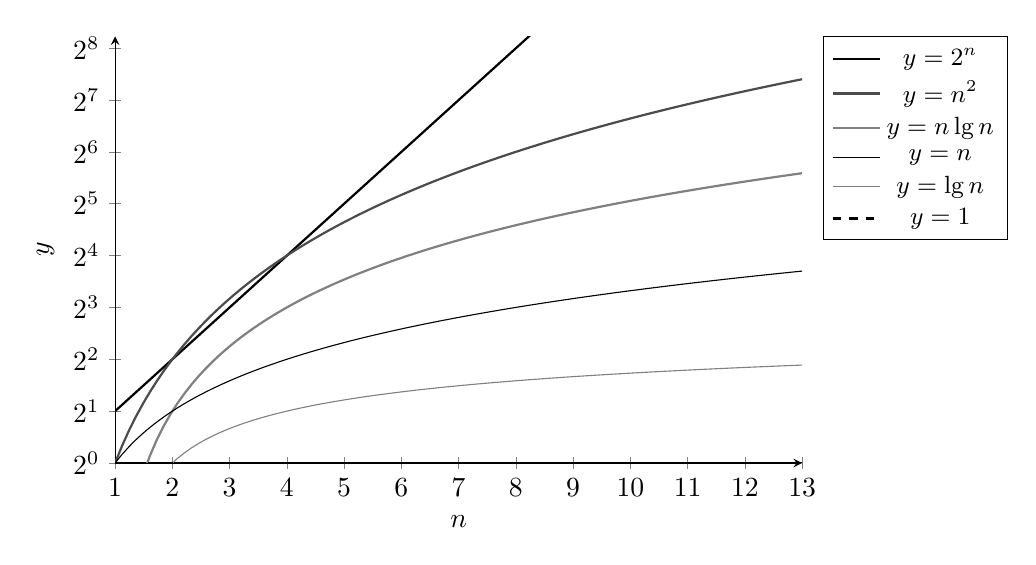
\begin{tikzpicture}
\begin{axis}[
    width=0.85\textwidth,
    height=7cm,
    xlabel={$n$},
    ylabel={$y$},
    xmin=1, xmax=13,
    ymin=1, ymax=300,
    ymode=log,
    log basis y=2,
    ytick={1,2,4,8,16,32,64,128,256},
    xtick={1,2,3,4,5,6,7,8,9,10,11,12,13},
    axis lines=left,
    legend pos=outer north east,
    legend style={font=\small},
    every axis plot/.append style={thick},
]
\addplot[domain=1:9, samples=100, black, thick] {2^x};
\addlegendentry{$y = 2^n$}

\addplot[domain=1:13, samples=100, black!70, thick] {x^2};
\addlegendentry{$y = n^2$}

\addplot[domain=1:13, samples=100, gray, thick] {x*ln(x)/ln(2)};
\addlegendentry{$y = n \lg n$}

\addplot[domain=1:13, samples=100, black, thin] {x};
\addlegendentry{$y = n$}

\addplot[domain=1:13, samples=100, gray, thin] {ln(x)/ln(2)};
\addlegendentry{$y = \lg n$}

\addplot[domain=1:13, samples=2, black, dashed] {1};
\addlegendentry{$y = 1$}
\end{axis}
\end{tikzpicture}
\caption{Crecimiento de algunas funciones comunes en la complejidad computacional.}
\label{fig:crecimiento}
\end{figure}

\begin{ejemplo}
Encuentre una notación $\Theta$ para el número de veces que se ejecuta la asignación $x = x + 1$ en el siguiente algoritmo.

\begin{lstlisting}
j = n
while (j >= 1) {
    for i = 1 to j
        x = x + 1
    j = floor(j/2)
}
\end{lstlisting}

\textbf{Solución.}
\[
T(n) = n + \left\lfloor \frac{n}{2} \right\rfloor + \left\lfloor \frac{n}{4} \right\rfloor + \cdots + \left\lfloor \frac{n}{2^{k-1}} \right\rfloor
\]
donde $k$ denota el número de veces que se ejecuta el cuerpo del ciclo \texttt{while}, es decir, el número de veces que se ejecuta $x = x + 1$.

Acotando superiormente:
\[
T(n) \leq n + \frac{n}{2} + \frac{n}{4} + \cdots + \frac{n}{2^{k-1}}
= \frac{n\left(1 - \frac{1}{2^k}\right)}{1 - \frac{1}{2}}
= 2n\left(1 - \frac{1}{2^k}\right) \leq 2n
\]
luego $T(n) = O(n)$. Además, como cada término es positivo,
\[
T(n) \ge n \quad \Rightarrow \quad T(n) = \Omega(n)
\]
Por lo tanto,
\[
T(n) = \Theta(n)
\]
\end{ejemplo}

\begin{observacion}
Un problema se considera \textbf{tratable} o factible cuando existe un algoritmo que lo resuelve con un tiempo de ejecución polinomial en el peor de los casos. Esta condición se interpreta como la posesión de una solución eficiente. No obstante, si el tiempo requerido es proporcional a un polinomio de grado elevado, la solución podría ser ineficiente en la práctica. Afortunadamente, en muchos casos de importancia, el grado del polinomio que acota el tiempo de ejecución es bajo, lo que garantiza una verdadera eficiencia.

Se denomina \textbf{intratable} a un problema para el cual no se conoce ningún algoritmo que lo resuelva en tiempo polinomial en el peor caso. Esto implica que cualquier algoritmo que lo solucione requerirá un tiempo de ejecución prohibitivamente largo, generalmente de naturaleza exponencial o factorial, incluso para instancias o entradas de tamaño moderado.

Se dice que un problema es \textbf{irresoluble} o no computable cuando no existe ningún algoritmo capaz de resolverlo. Un ejemplo fundamental, y uno de los primeros en ser demostrado como tal, es el problema de la parada\footnote{Halting problem.}: determinar si un programa cualquiera se detendrá en algún momento, dada una entrada específica. Existe una variedad significativa de problemas de este tipo, varios de los cuales revisten gran importancia práctica en el campo de la computación teórica.

Existe una gran cantidad de problemas computacionales solucionables cuyo estatus de complejidad permanece indeterminado; si bien se conjetura que son intratables, aún no se ha demostrado formalmente que lo sean. La mayoría de estos problemas pertenecen a la clase de los NP-completos.
\end{observacion}